\documentclass[22pt,handout]{beamer}
% \documentclass[handout]{beamer}
% add theme and color theme https://www.overleaf.com/learn/latex/Beamer#Reference_guide
\setbeamertemplate{navigation symbols}{arguments} % hides navigation buttons
\setbeamertemplate{footline}[frame number]
\usepackage[utf8]{inputenc}
\usepackage{minted}
\usepackage{graphicx}
\usepackage{comment}
%% \usepackage[b]{beamer}
\usemintedstyle{tango}
\pagenumbering{roman}

\title{Docker something}
\author{Julia Winkler}
\date{19.06.2024}

\begin{document}

%% TODO: layout element, dass kennzeichnet, wann man ins terminal wechselt vgl. "Vorlesung" bei EAE
%% TODO: how to make one list item without overhead -> macro?
%% TODO: oneline minted

\begin{frame}[t]
    \vfill
    \begin{center}
        
\includegraphics[width=1\textwidth]{Bilder/docker-how.png}
    \end{center}
    \vfill
\end{frame}

\maketitle

\begin{frame}{Gliederung}
    \tableofcontents
\end{frame}

\begin{frame}
    \frametitle{Wiso, Weshalb, Warum?}
    \begin{center}
        
\includegraphics[width=0.8\textwidth]{Bilder/docker-why.png}
    \end{center}\pause
    \begin{center}
        "a sandboxed process on your machine that is isolated from all other processes on the host machine"
    \end{center}\pause
    \begin{center}
        "It works on my computer"
    \end{center}\pause
    \begin{center}
        "faster onboarding and testing while also simplifying the deployment of services"
    \end{center}
\end{frame}

\begin{frame}[t]
    \frametitle{Wer ist Moby Dock?}\pause
    \only<2>{\begin{figure}[h]
        \centering
        
\includegraphics[width=0.8\textwidth]{Bilder/mobydocker.jpg}
    \end{figure}
    }
    \only<3>{\begin{figure}[h]
        \centering
        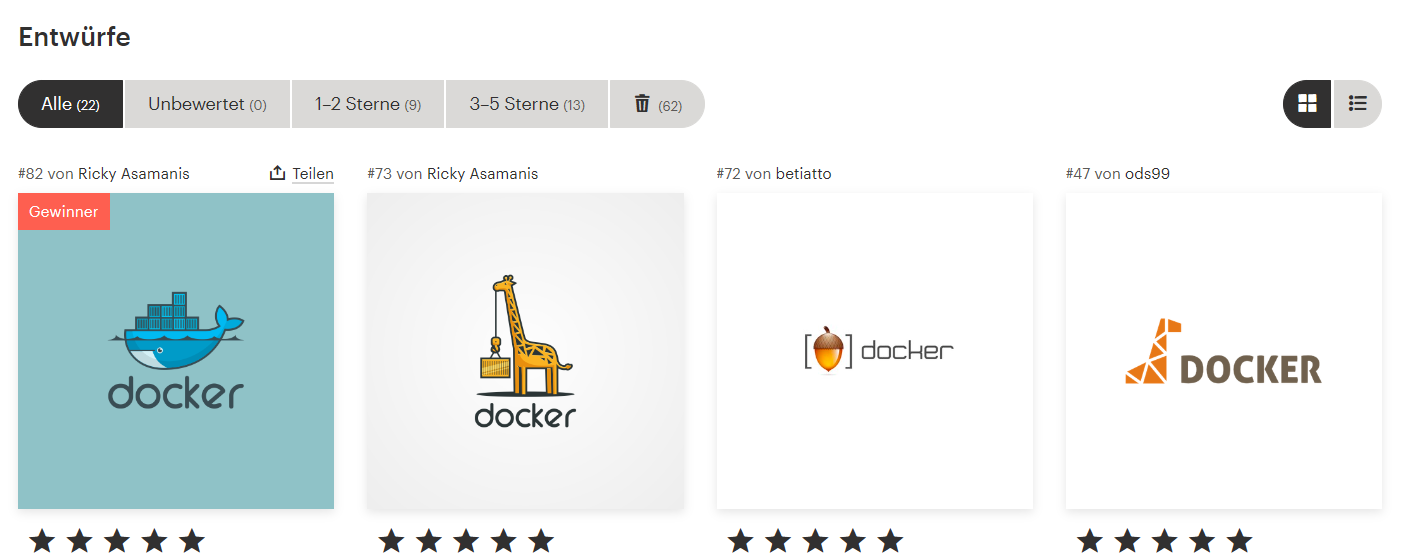
\includegraphics[width=0.8\textwidth]{Bilder/wettbewerb.png}
        \caption{Wettbewerb zum Icon für Docker}
    \end{figure}
    }
\end{frame}

\begin{frame}[t]
    \frametitle{Was ist Docker?}
    %% TODO: good definition or leave out
    \begin{itemize}
        \item ? (vllt nicht als Folie sondern nur was erwähnen)
        \item Toolbox
        \item sandbox
        \item configurierbare Umgebung
    \end{itemize} 
    %% bild
    \begin{figure}[h]
        \centering
        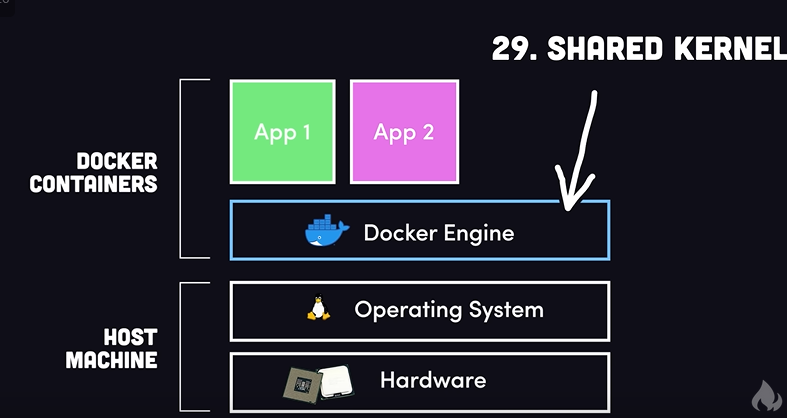
\includegraphics[width=0.5\textwidth]{Bilder/Docker Concept.png}
    \end{figure}
\end{frame}

\begin{frame}[t]
    \frametitle{Was ist Docker?}
    \begin{figure}[h]
        \centering
        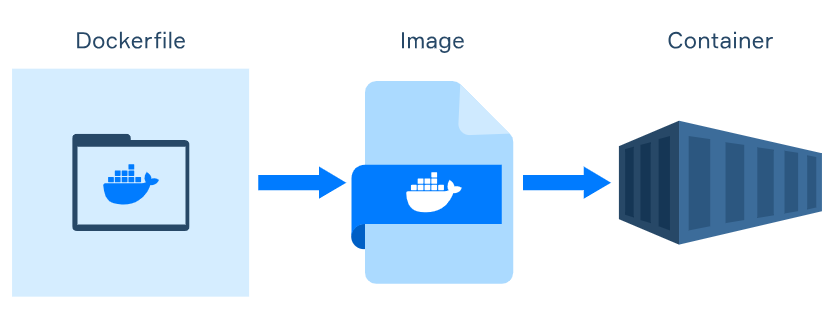
\includegraphics[width=0.5\textwidth]{Bilder/Docker-Ablauf.png}
        \caption{Zusammenhang der Docker Komponenten}
    \end{figure}
\end{frame}

\begin{frame}[t]
    \frametitle{Wichtige Begriffe}
    %% TODO: good formatting for this slide
    Docker
    - freie Software zur Isolierung von Anwendungen mit Hilfe von Containervirtualisierung
    Container
    - Umgebung in der die tatsächliche Anwendung läuft
    Image
    - Blaupausen, um einen Container zu erstellen
    Dockerfile
    - Anleitung, um ein Image zu erstellen
    Docker Compose
    - Orchestrierungstool (?), Wrapper für einen oder mehrere Container
    Container Registy (Docker Hub) 
    - Ort an dem viele verschindene Images gespeichert und geteilt werden können
    Docker Desktop
    - UI für alles was man in der CLI machen kann (?) %% TODO: 
\end{frame}

\begin{frame}[t]
    \frametitle{Wie kreige ich dieses "Docker"?}
    %% TODO: installation guide + ref to docker desktop
\end{frame}

\begin{frame}[fragile]
    \frametitle{Hello World} %% winkende Hand?
    \begin{minted}{bash}
        $ docker -v
        $ docker --help
        $ docker run hello-world
    \end{minted}

    Ab ins Terminal
\end{frame}

\begin{frame}[t]
    \frametitle{Was ist Docker?}
    %% TODO: highlight so that dockerfile is highlighted
    \begin{figure}[h]
        \centering
        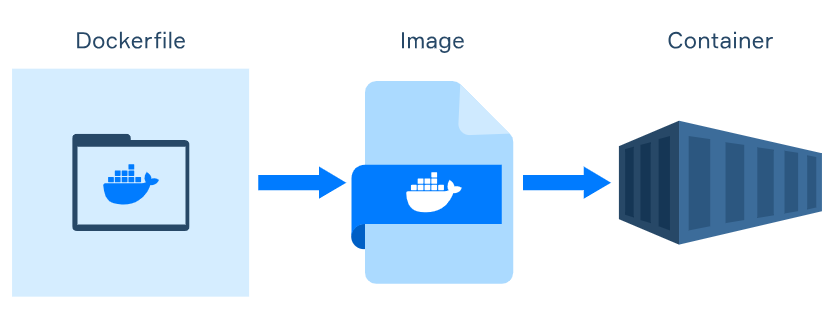
\includegraphics[width=0.5\textwidth]{Bilder/Docker-Ablauf.png}
        \caption{Zusammenhang der Docker Komponenten}
    \end{figure}
\end{frame}

\begin{comment}
    \begin{frame}[t]
    \frametitle{Basic commands}
    \begin{itemize}
        \item docker run
        \item docker ps / docker ps -a
        \item 
    \end{itemize} 
\end{frame}
\end{comment}


\begin{frame}[t]
    \frametitle{Dockerfile}
    \begin{itemize}
        \item Ein Dockerfile ist die Anleitung um ein Image zu erstellen.
        %% Mit einem Dockerfile kann man den Inhalt des Containers configurieren
        %% \item Image zu einem Dockerfile erstellen: \verb|docker build .|
        %%\item Image mit einem namen versehen: \verb|-t name:version| (version ist optional)
        \item Standardmäßig hießt die Datei 'Dockerfile'
        %%\item \verb|-f <Dateiname>| für eigens benannte Dateien
    \end{itemize}

    \verb|make lc-line-concept|
    
    %% TODO: Image zu Hello World ?
    \begin{figure}[h]
        \centering
        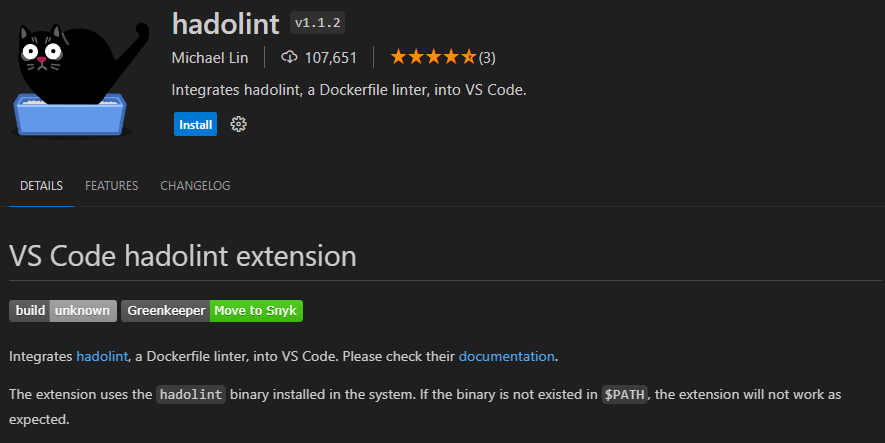
\includegraphics[width=0.5\textwidth]{Bilder/Hadolint.png}
        \caption{Plugin für die Arbeit mit Docker}
    \end{figure}

\end{frame}

%% Ü: Wie sieht also ein Dockerfile aus
\begin{frame}[t]
    \frametitle{Dockerfile}
    %% Code tour durch ein Dockerfile mit allen Elementen oder hier eines langsam aufbauen
    \inputminted[fontsize=\footnotesize, frame=lines]{dockerfile}{../examples/Dockerfile}
    \begin{itemize}
        \item FROM, CMD \& Entrypoint, RUN, COPY, ARG
        \item Layer %% TODO: one per command?
    \end{itemize} 
\end{frame}

\begin{frame}[fragile]
    \frametitle{title}
    \begin{minted}{bash}
        docker build -t example:cmd -f Dockerfile.cmd .
        docker build -t example:entry -f Dockerfile.entry .

        docker run example:cmd
        docker run example:cmd hello
        docker run example:entry hello
    \end{minted}
\end{frame}

\begin{frame}[fragile]
    \frametitle{title}
    \begin{minted}{bash}
        docker build -t example:single -f Dockerfile.single .
        docker build -t example:multi -f Dockerfile.multi .

        docker ps -a
        docker images
    \end{minted}
\end{frame}
%% vllt Docker mit ubuntu for exec, it, start, stop, name

\begin{frame}[fragile]
    \frametitle{Python bsp}
    \inputminted[fontsize=\footnotesize, frame=lines]{dockerfile}{../examples/Dockerfile.cmd}
    %% run mit volume und port
    %% start, stop, rm
\end{frame}

\begin{frame}[t]
    \frametitle{Volumes}
    \begin{itemize}
        \item 
    \end{itemize} 
\end{frame}

\begin{frame}[fragile]
    \frametitle{React}
    \inputminted[fontsize=\footnotesize, frame=lines]{dockerfile}{../examples/Dockerfile.cmd}
\end{frame}

\begin{frame}[t]
    \frametitle{Multistage builds}
    \begin{itemize}
        \item 1
    \end{itemize} 
\end{frame}

\begin{frame}[fragile]
    \frametitle{React - Multistage}
    \inputminted[fontsize=\footnotesize, frame=lines]{dockerfile}{../examples/Dockerfile.cmd}
\end{frame}

\begin{frame}[t]
    \frametitle{Dockerfile Best practices}
    \begin{itemize}
        \item RUN commands
        \item Order of COPY
        \item Volumes
        \item Multistage
    \end{itemize} 
\end{frame}

\begin{frame}[t]
    \frametitle{Docker Compose}
    \begin{itemize}
        \item Vorteile
        \item UseCases
    \end{itemize} 
\end{frame}

\begin{frame}[fragile]
    \frametitle{Docker Compose zu Python}
    \inputminted[fontsize=\footnotesize, frame=lines]{dockerfile}{../examples/Dockerfile.cmd}
\end{frame}

\begin{frame}[fragile]
    \frametitle{Docker Compose Webapp}
    \inputminted[fontsize=\footnotesize, frame=lines]{dockerfile}{../examples/Dockerfile.cmd}
\end{frame}

\begin{frame}[t]
    \frametitle{important Commands}
    \begin{itemize}
        \item docker run
        \item docker build
        \item docker push, pull
        \item docker ps -a
        \item docker rm / rmi
        \item ...
    \end{itemize} 
\end{frame}

\begin{frame}[t]
    \frametitle{Coole Quellen und so weiter}
    \begin{itemize}
        \item \href{https://www.docker.com/}{https://www.docker.com/}
        \item \href{https://docs.docker.com/get-started/}{https://docs.docker.com/get-started/}
        \item 
    \end{itemize} 
\end{frame}

\begin{comment}

\begin{frame}[t]
    \frametitle{title}
    \begin{itemize}
        \item 1
    \end{itemize} 
\end{frame}

\begin{frame}[fragile]
    \frametitle{title}
    \inputminted[fontsize=\footnotesize, frame=lines]{dockerfile}{../examples/Dockerfile.cmd}
\end{frame}

\begin{wrapfigure}{l}{0.25\textwidth}
    \centering
    \includegraphics[width=0.25\textwidth]{contour}
\end{wrapfigure}

\begin{figure}[h]
    \centering
    \includegraphics[width=0.5\textwidth]{spiral}
    \caption{}
\end{figure}
    
\end{comment}

\end{document}